\documentclass[10pt,a4paper]{article}			%format de page
\usepackage[utf8]{inputenc}						%encodage avec caractères accentués
\usepackage[T1]{fontenc}						%encodage
\usepackage[english,frenchb]{babel}						%typographie française
\usepackage{fancyhdr}
\usepackage{lastpage}
\usepackage{graphicx}
\usepackage{amsmath}
\usepackage{amsfonts,amssymb}
% Mise en page
\usepackage{geometry}
\geometry{a4paper,twoside,left=2.5cm,right=2.5cm,top=2.8cm,bottom=2.8cm} %taille et marges
\pagestyle{fancy}								%style de page {fancy(package), empty, plain, headings}
\renewcommand{\headrulewidth}{0pt}				%épaisseur du trait de tête de page (0.4pt)
\fancyhead[L]{}									%pied de page gauche
\fancyhead[C]{}									%pied de page centre
\fancyhead[R]{}									%pied de page droit
\renewcommand{\footrulewidth}{0pt}				%épaisseur du trait du pied de page (0.4pt)
\fancyfoot[L]{}									%pied de page gauche
\fancyfoot[C]{}									%pied de page centrce
\fancyfoot[R]{\thepage{}/\pageref{LastPage}}	%pied de page droit

\thispagestyle{empty}				% Page de garde vide

% Infos générales
\title{Symmetry Detection}
\author{Chantal DING, Chloé MACUR}
\begin{document}

\selectlanguage{english}

\thispagestyle{empty}							%page de garde vide
%\begin{document}
	\begin{center}
		\hfill
		Chantal \bsc{Ding}
		\hfill \hfill
		Chloé \bsc{Macur}
		\hfill ~
		\par
		\noindent
		\\
		\vspace{0.7cm}
		\textit{December 2013}
		\vfill\vfill
		\Huge
		\begin{tabular}{c}
			\hline
			%Projet\\
			{\Large{\textsc{Symmetry Detection}}}\\
			~~~A Planar-Reflective Symmetry\\ Transform for 3D Shapes~~~\\
			\hline
		\end{tabular}
		\large
		\vfill
		 Project report\\
		 INF555 -- Digital Representation and Analysis of Shapes
	\end{center}
	\vfill
	\begin{flushright}
	
\includegraphics[scale=0.1]{img/logo_x_h.jpg}
	\end{flushright}
	\newpage 
\newpage
\tableofcontents

\newpage
	
	\section*{Introduction}
\addcontentsline{toc}{section}{Introduction}
  
	A lot of 3D shapes, whether natural or man-made, present some kind of symmetry that can be really useful in computer vision and 3D geometry.  Indeed symmetries allow certain economy, especially in digital representation, but they are also involved in pattern recognition or geometry completion. Thus, numerous methods are used to detect symmetries, partly because of the diversity of datas (point clouds, polygon meshes, NURBS, patches, etc.).  
 
	\section{A Planar-Reflective Symmetry Transform for 3D Shapes}
	
		%TODO delete before saving
	\textit{· 1 page description of the method you're implementing. (A Planar-Reflective Symmetry Transform for 3D Shapes paper) It goes without saying that you shouldn't copy text from the paper, but rather describe in your own words what the method is trying to do and how it does it. \\}
	
	We chose to try to implement the planar reflective symmetry transform (PRST) described by Podolak et al. ~\cite{Podolak:2006:APS}.
	
	Monte Carlo évite brute force, sélection intelligente selon l'énergie de la fonction
	
	\section{Our implementation}
	
	%TODO delete before saving
	\textit{· 2 page description of your implementation. Here you should describe the main building blocks of your implementation. We are especially interested in: whether you had any problems, whether there were things not mentioned in the paper that you had to discover or derive yourself (be very explicit about your own work!), whether you used any external libraries, etc. What we're not interested in: what are the names of your classes and variables, what operating system you were using, if you had to change some header files, etc. Whenever possible (which is most of the time), please try to use images instead of text to explain concepts.\\
	Your project should include some amount of independent work, either by implementing a technique and showing its performance on some examples not included by the authors, or by doing some independent theoretical analysis.\\}

	\subsection {Conventions et Notations}
We chose to use .png images as input files as they are naturally rasterized and do not typically have artefacts. For more simplicity we only considered grayscale images. Since the method we are implementing is taking advantage of sparsity in the function, a typical input image would be a black and white outline (see Figure \ref{exemple_carre}). The Java class \texttt{BufferedImage} provides an easy way to access such images and manipulate them as arrays of integers between 0 and 255. 
\begin{figure}[h]
\begin{center}

\includegraphics[scale=0.5]{img/carre.png}
\caption{Example of input image}
\label{exemple_carre}
\end{center}
\end{figure}

Since pixel values are high for white and low for black, we want to work with the function $f$ defined as follows for each pixel $p$ of the image $I$ :
\[f(p) = 255 - \text{intensity of $I$ at $p$}\]
so that $f(p)=0$ for white pixels, i.e. empty space.

For point coordinates, we simply use the default Java coordinate system, with $(0,0)$ in the upper-left corner, as shown in Figure \ref{coordinates}. All points have integer coordinates. Lines however, are parametrized over a pair of \texttt{double} values $(r,\theta)$ where $r$ is the distance of the line to the origin and $\theta$ the angle of the normal vector, as shown in Figure \ref{lines_parametrization}.
\begin{figure}[h]
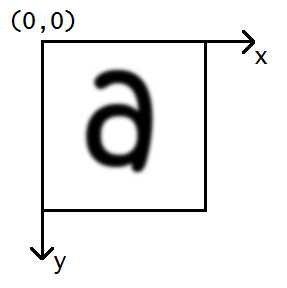
\includegraphics[scale=0.5]{img/coordinates.png}
\caption{$(x,y)$ coordinates for Java images}
\label{coordinates}
\end{figure}
\begin{figure}[h]
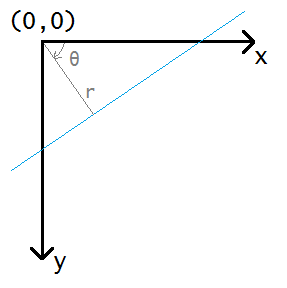
\includegraphics[scale=0.7]{img/lines.png}
\caption{$(r,\theta)$ parametrization of lines}
\label{lines_parametrization}
\end{figure}


	\subsection{Sampling}
In order to compute the PRST using the Monte Carlo algorithm for sparse functions, we first perform an importance sampling of points in the image, using $f(x)$  as the probability density of selecting $x$. For this, we use the cumulative sum of $f(x)$ over the image as the cumulative distribution function and perform an inverse transform sampling. Usually, this method works by generating a real number $u$ in range [0,1] and computing $F^{-1}(u)$, where $F$ is a cumulative distribution function. Here, we adapted the method to work with non-normalized integer functions :
\begin{enumerate}
\item Generate a random integer n in range $[0,max_F]$, where $F$ is the cumulative sum of pixel values and $max_F$ its maximum value;
\item Let $p_1,...,p_N$ be the pixels of the image, compute $i=\inf\{m\in \mathbb{N}, m\leq N |  F(p_m) = n\}$;
\item Add $p_m$ to the sample.
\end{enumerate}



	\subsection{Adjustments for 2D}
	
	the polar issue, formulas different, etc...

The Monte Carlo algorithm we chose to use for computing the PRST requires to derive a change-of-variable weight for each pair of points $(x,x')$, accounting for the transformation between the discrete parametrization of lines over $(r,\theta)$ and the pairs of reflected points. In 3D, the change-of-variables weight is given by the following formula :
\[w_{change-of-variables} = 2d^2\sin\theta\]
However, since we are working in 2D, we need to recompute this weight in order to fit the new coordinates system. As in 3D, we compute the determinant of the Jacobian of the change-of-variables transformation. Let 
\[\vec{n}=\begin{pmatrix}\cos\theta \\ \sin\theta\end{pmatrix}\]
be the normal of the line of reflection, $d$ the distance between $x$ and $x'$, we can write :
\begin{align*}
 d & = \lVert x-x' \rVert  \\
& = 2(r-\vec{n}\cdot x) \\
x' &= x+ d\vec{n}\\
&= x+ 2(r\vec{n} - (\vec{n}\cdot x)\vec{n})
\end{align*}
thus we have :
\begin{align*}
\frac{\partial x'}{\partial r}&=2\vec{n}\\
\frac{\partial x'}{\partial \theta}&= 2r\vec{u}-2[(\vec{u}\cdot x)\vec{n}+(\vec{n}\cdot x)\vec{u}]
\end{align*}
where 
\[\vec{u}=\frac{\partial \vec{n}}{\partial \theta} = \vec{n}=\begin{pmatrix}-\sin\theta \\ \cos\theta\end{pmatrix}.\]
Therefore, the Jacobian is
\[J = 2
\begin{pmatrix}
\cos\theta & -r\sin\theta-(\vec{u}\cdot x)\cos\theta+(\vec{n}\cdot x)\sin\theta\\
\sin\theta &  r \cos\theta - (\vec{u}\cdot x)\sin\theta - (\vec{n}\cdot x)\cos\theta
\end{pmatrix}\]
and so the determinant is
\[w_{change-of-variables} = |J| = 2d.\]

  	\subsection{Comments}
  	Choice of the 1/N factor in the calculus of D : explain that it comes out of the blue ... \\
  	
  	Bounds : la valeur du prst (monte carlo) obtenue telle qu'on le fait dépend complètement de l'unité de longueur qu'on utilise pour calculer les distance x,x'. Du coup on n'a vraiment aucune garantie sur les bornes du prst Monte Carlo, contrairement au prst complet...\\
  	
  	
  	\section{Results}
  		%TODO delete before saving
\textit{· 1.5-2 pages of results. Show (especially in, graphs, screenshots, etc.) the results that you have obtained. Comment on discrepancies (if any) with the results shown in the paper. Comment on whether you had to tweak parameters to get good results and, if so, how you picked them.\\}

	\section{Possible extensions}
	
\textit{· 0.5-1 pages of possible extensions. Can you suggest how the method can be improved? Can you suggest other application domains for your method?\\}

	\section*{Conclusion}
\addcontentsline{toc}{section}{Conclusion}

\addcontentsline{toc}{section}{References} 
\nocite{*}
\bibliographystyle{plain}
\bibliography{bibli}
		
\end{document}
